\documentclass[12pt]{article}
\usepackage[utf8]{inputenc}
\usepackage[margin=1in]{geometry}
\usepackage[final]{graphicx}
\usepackage{stickstootext}
\usepackage{lastpage}
\usepackage[stickstoo,vvarbb]{newtxmath}
\usepackage{fancyhdr}

\pagestyle{fancy}
\fancyhf{}
\fancyfoot{}
    \fancyfoot[R]{Page \thepage\ of \pageref{LastPage}}
\rhead{Documentation}
\lhead{Oof}
\renewcommand{\headrulewidth}{0.5pt}
\renewcommand{\footrulewidth}{0.5pt}

\begin{document}
    \title{\vspace{0mm}\textbf{Documentation}}
    \date{\vspace{-10mm}September 19, 2020}
    \maketitle

\begin{center}
    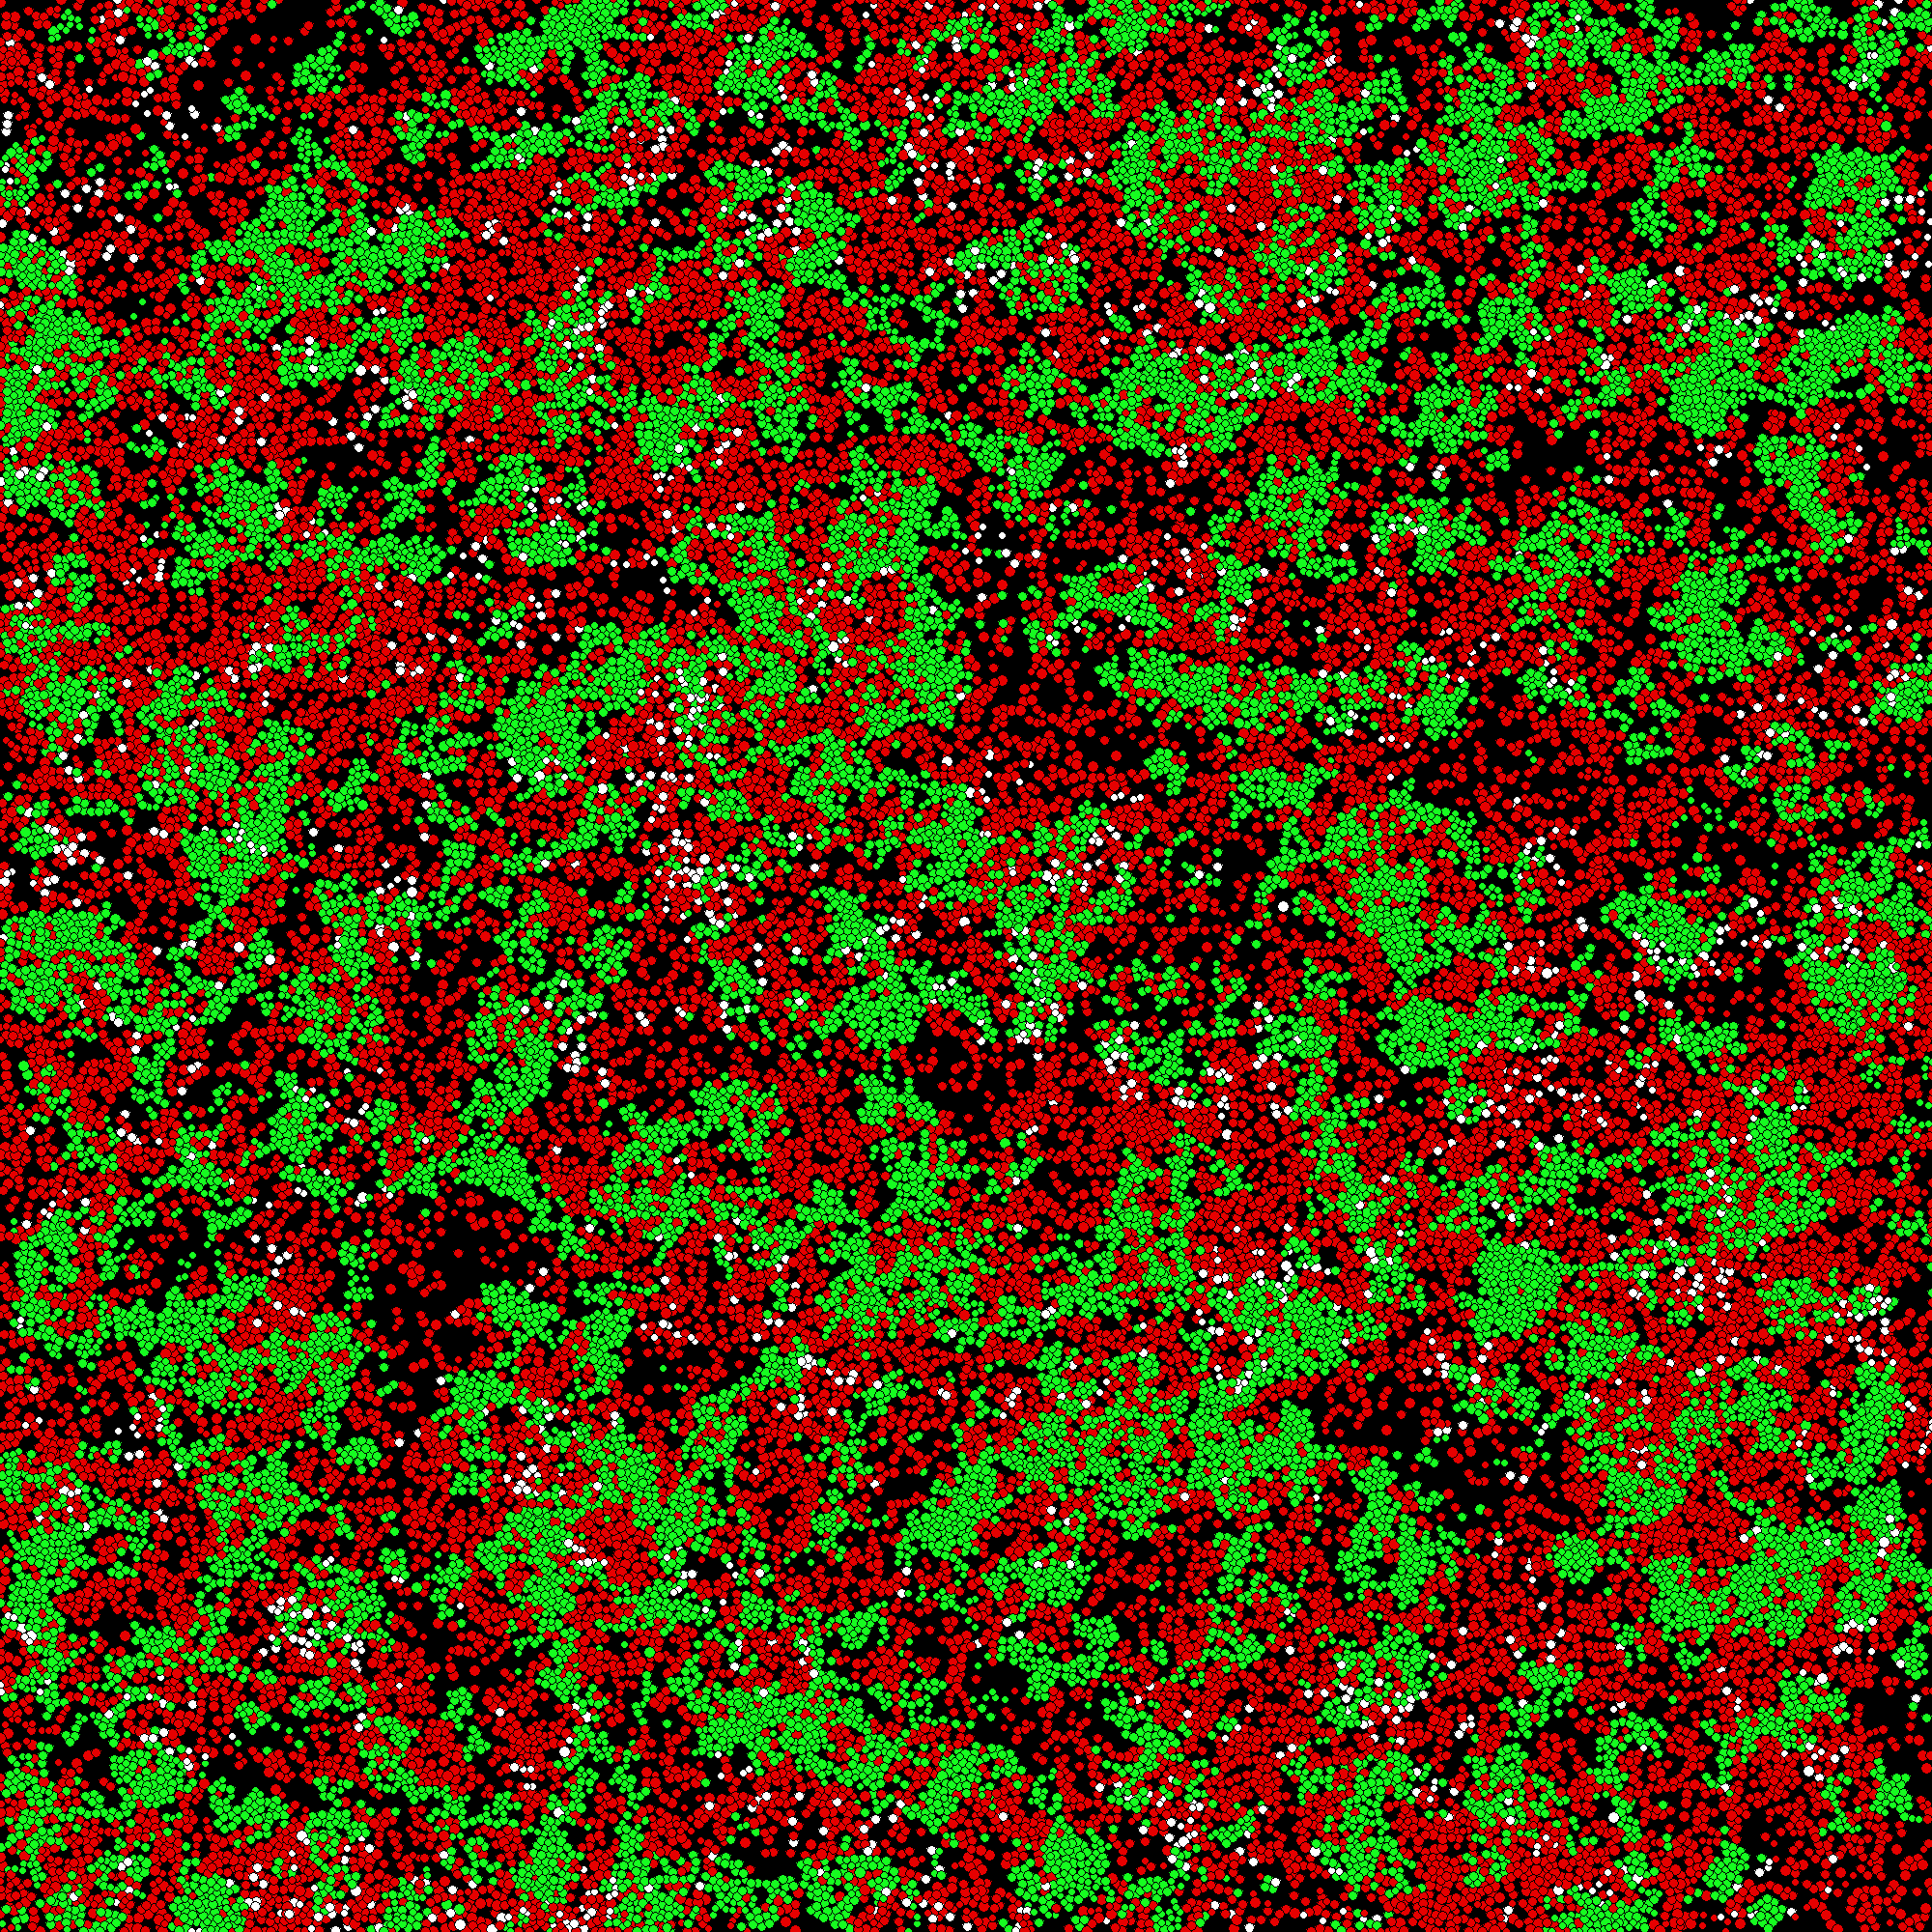
\includegraphics[width=15cm]{../images/front_page.png}
\end{center}

\newpage

\tableofcontents

\newpage

    \section{Introduction}\label{sec:intro}

    \section{Installation}\label{sec:install}

    \section{Input}

    \section{Johnson-Kendall-Roberts theory}\label{sec:jkr}

    \subsection{Spherical implementation}\label{subsec:sphere}

    \subsection{Ellipsoidal implementation}\label{subsec:ellipse}

    \section{Fixed-radius neighbor search}\label{sec:fixed}

    \section{Output}

    \section{Imaging}\label{sec:imaging}

    \subsection{Imaging in 2D}\label{subsec:2d}

    \subsection{Imaging in 3D}\label{subsec:3d}

    \section{Thanks}

\end{document}
